\subsection{Hypothesis 1}
\begin{center}
\centering
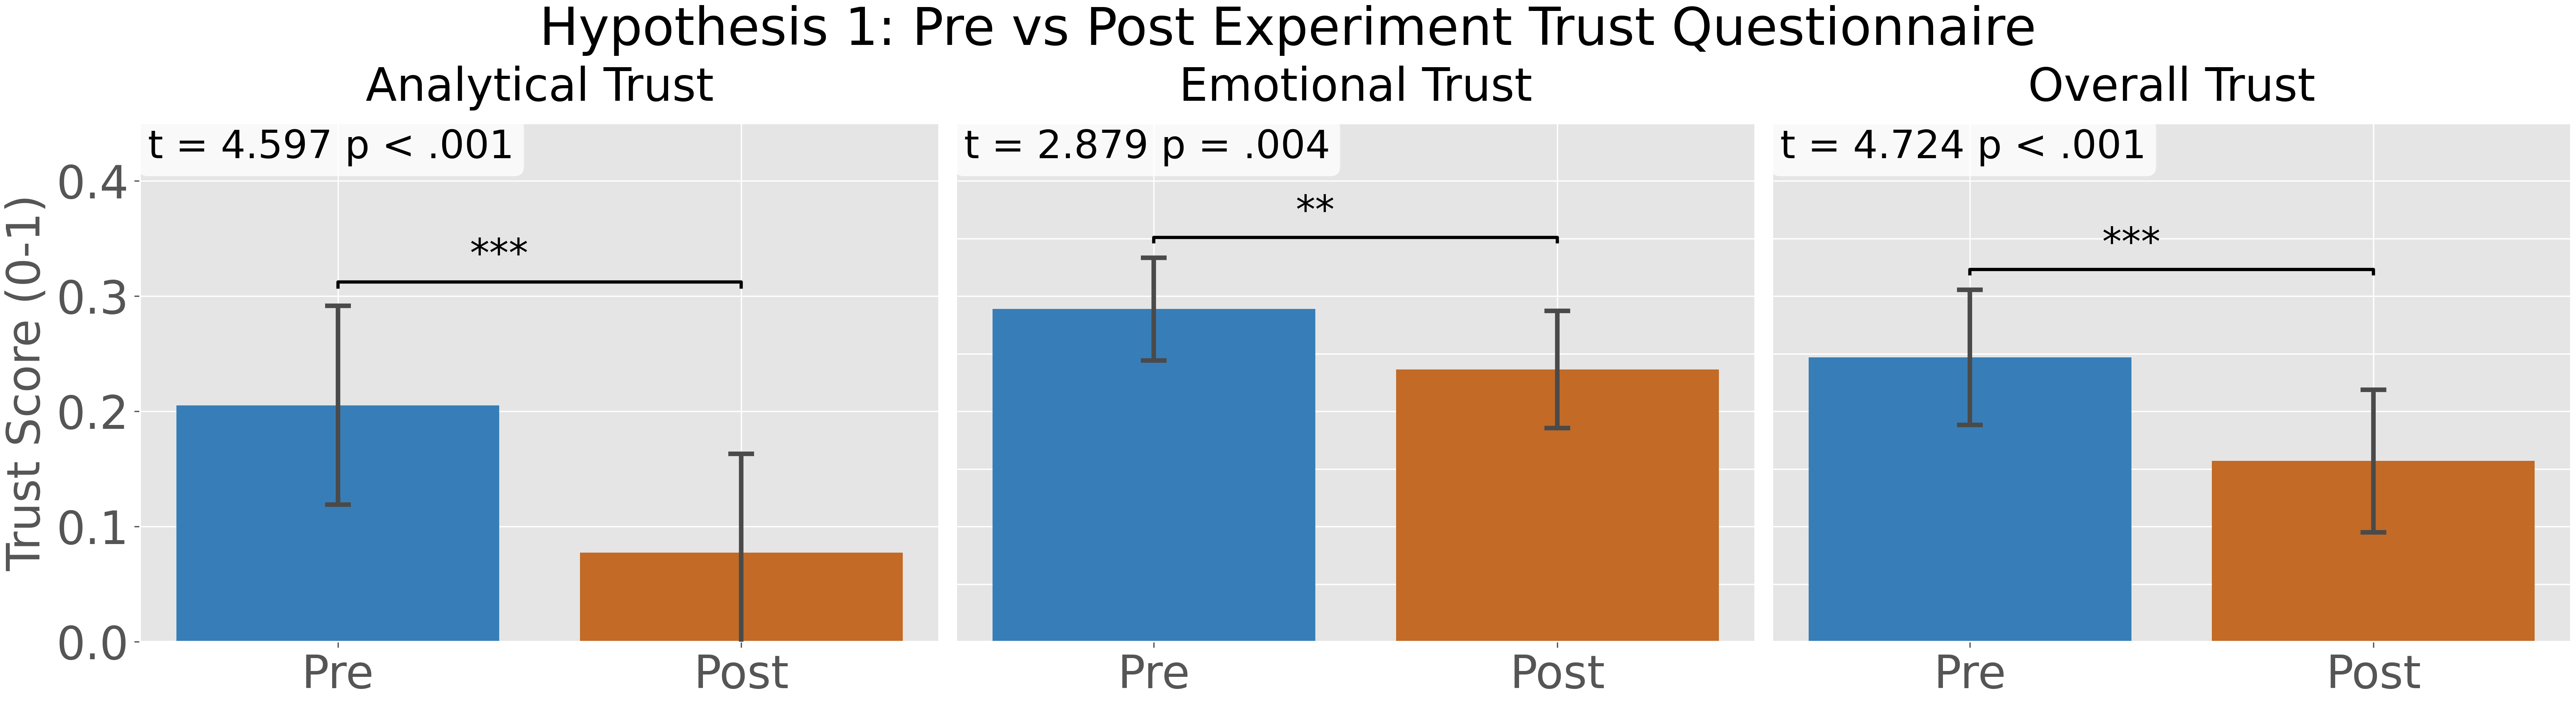
\includegraphics[width=\linewidth]{Figures/hypothesis1.png}

\captionof{figure}{Visualization for Hypothesis 1.}
\label{fig:hypothesis1}
\end{center}

Hypothesis 1 consisted of three sub-hypotheses that tested whether trust changed from pre- to post-experiment across overall, analytical, and emotional trust dimensions. Figure \ref{fig:hypothesis1} summarizes the pre-post means, and all analyses used paired-samples t-tests with two-sided Wilcoxon signed-rank tests as a robustness check. Across $454$ paired responses, overall trust decreased from $M_{pre}=0.247$ (95\% CI [0.188, 0.306]) to $M_{post}=0.157$ (95\% CI [0.095, 0.219]), $t(453)=4.724$, $p < .001$, $W=34761.500$, $p_{W} < .001$, $d=-0.222$, and $\Delta=-0.090$. Analytical trust showed the same pattern, declining from $M_{pre}=0.205$ (95\% CI [0.119, 0.292]) to $M_{post}=0.078$ (95\% CI [-0.008, 0.163]), $t(453)=4.597$, $p < .001$, $W=28342.000$, $p_{W} < .001$, $d=-0.216$, and $\Delta=-0.128$. Emotional trust also declined from $M_{pre}=0.289$ (95\% CI [0.244, 0.333]) to $M_{post}=0.236$ (95\% CI [0.185, 0.287]), $t(453)=2.879$, $p = .004$, $W=14885.000$, $p_{W} = .007$, $d=-0.135$, and $\Delta=-0.052$. After Benjamini-Hochberg correction, sub-hypotheses 1.1, 1.2, and 1.3 were significant. 

\subsection{Hypothesis 2}
\begin{center}
\centering
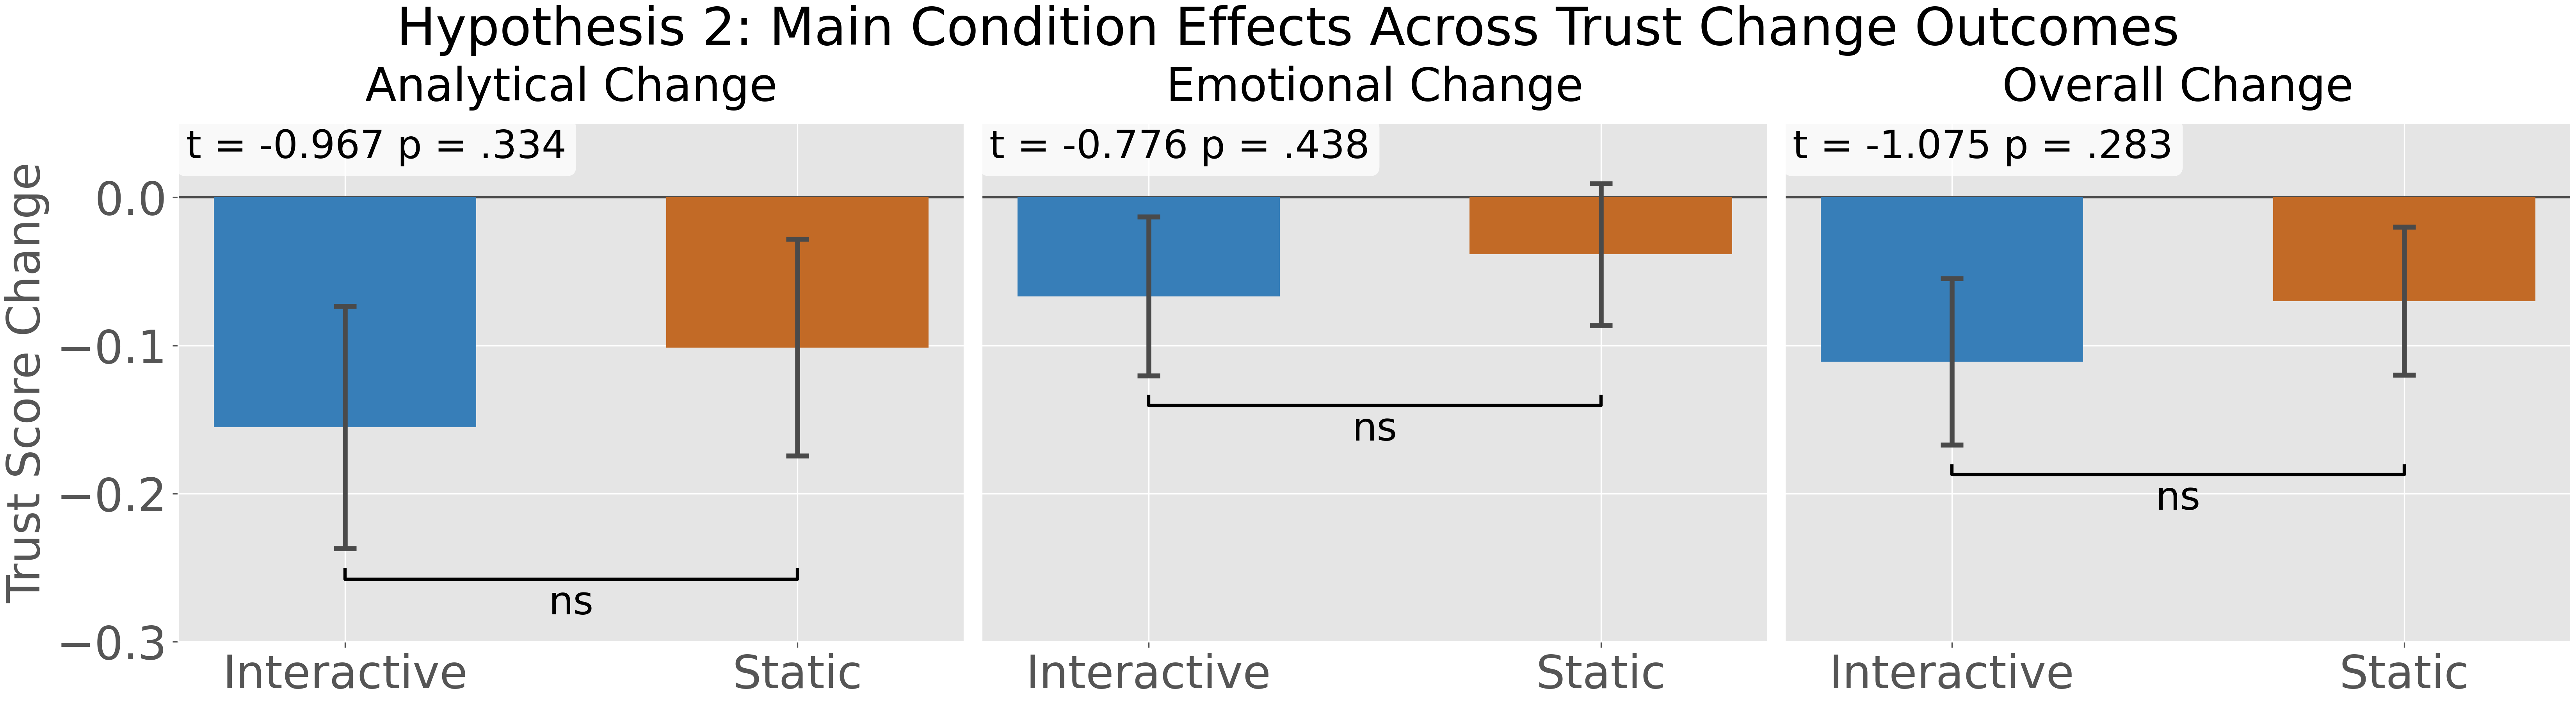
\includegraphics[width=\linewidth]{Figures/hypothesis2.png}

\captionof{figure}{Visualization for Hypothesis 2.}
\label{fig:hypothesis2}
\end{center}

Hypothesis 2 tested whether experimental condition changed the magnitude of trust change across overall, emotional, and analytical trust outcomes. Figure \ref{fig:hypothesis2} summarizes the mean change scores for the Interactive and Static conditions, and the primary analyses used Welch's two-sample t-tests to compare conditions for each outcome. Across $n_{Interactive}=223$ and $n_{Text}=231$ participants, overall trust change was $M_I=-0.111$ (95\% CI [-0.167, -0.055]) in the Interactive condition and $M_T=-0.070$ (95\% CI [-0.120, -0.020]) in the Static condition, Welch's $t(444.21)=-1.075$, $p = .283$, and $\Delta(M_I-M_T)=-0.041$. Emotional trust change followed the same pattern: $M_I=-0.067$ (95\% CI [-0.120, -0.013]) for Interactive participants and $M_T=-0.038$ (95\% CI [-0.086, 0.009]) for Static participants, Welch's $t(444.20)=-0.776$, $p = .438$, and $\Delta(M_I-M_T)=-0.028$. Analytical trust change also did not differ meaningfully by condition, with $M_I=-0.155$ (95\% CI [-0.237, -0.073]) in the Interactive condition and $M_T=-0.101$ (95\% CI [-0.175, -0.028]) in the Static condition, Welch's $t(444.81)=-0.967$, $p = .334$, and $\Delta(M_I-M_T)=-0.054$. After Benjamini-Hochberg correction, sub-hypotheses 2.1, 2.2, and 2.3 were not significant. We were additionally interested in whether there was a confounding effect of WEIRD vs. Normal cultural background, and performed a follow-up comparison of the effect of condition within cultural background. This comparison also showed no significant effect of condition and is reported in the supplementary materials. 

\subsection{Hypothesis 3}
\begin{center}
\centering
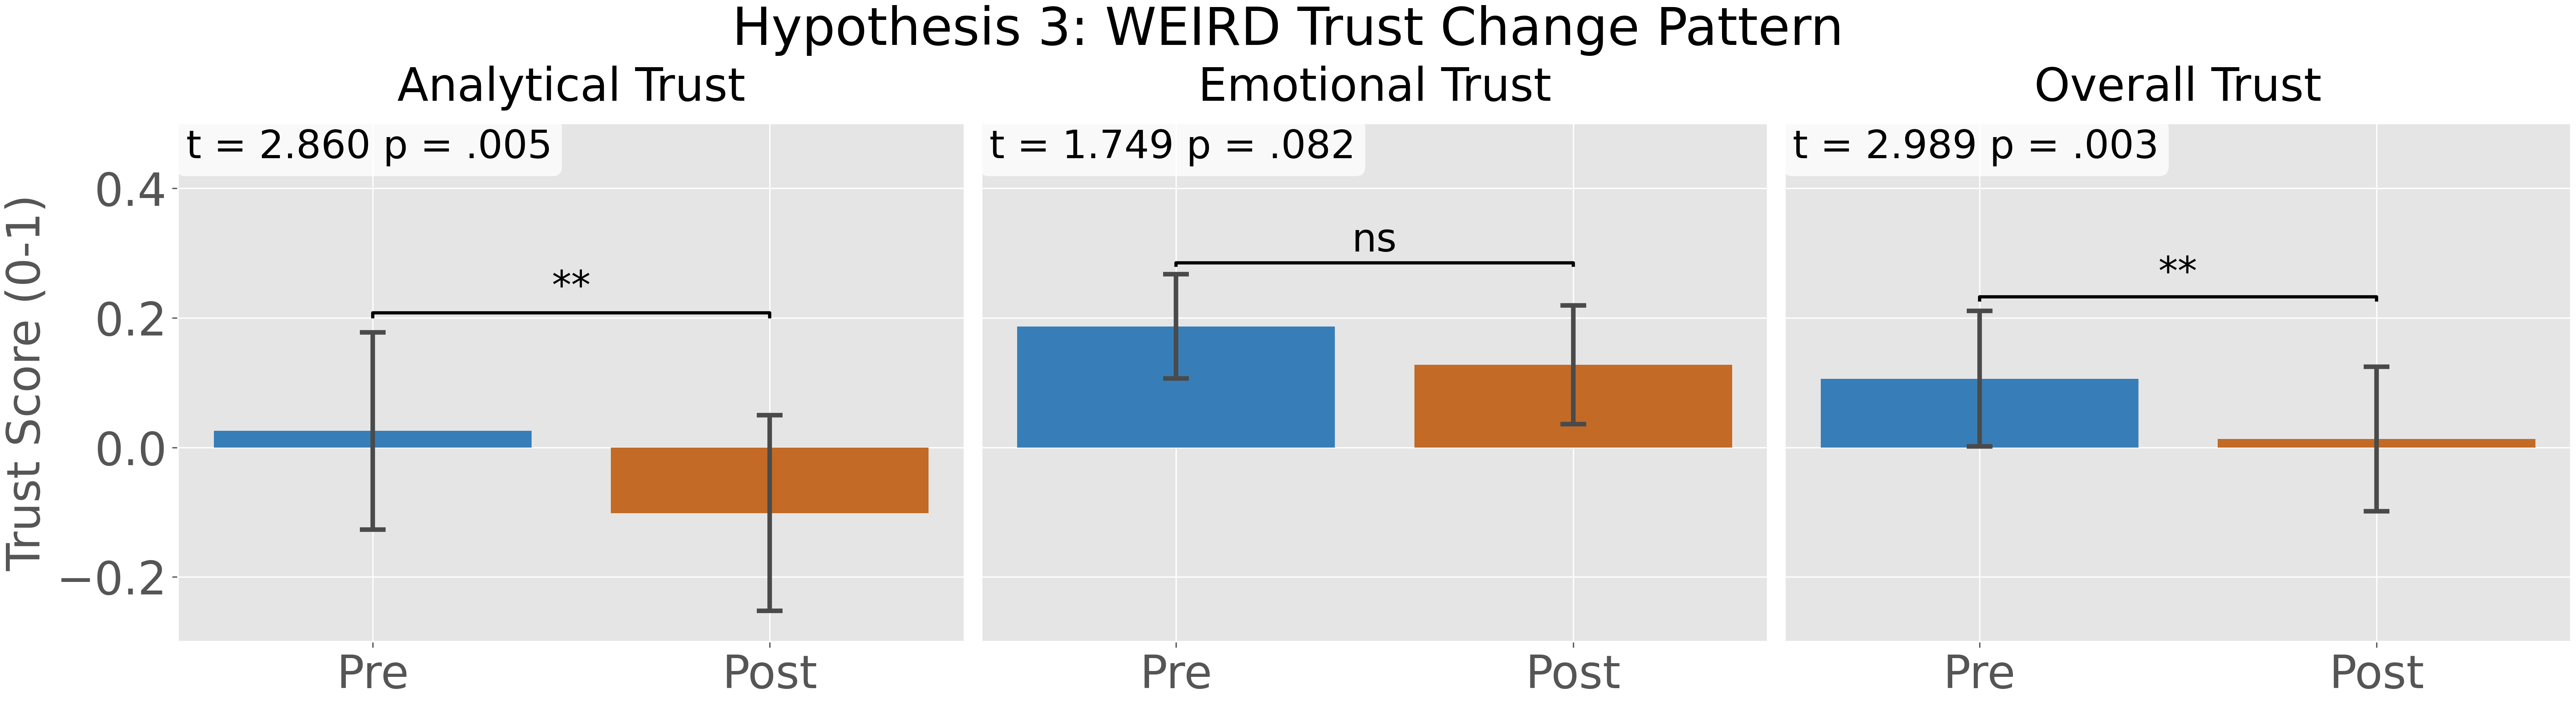
\includegraphics[width=\linewidth]{Figures/hypothesis3.png}

\captionof{figure}{Visualization for Hypothesis 3.}
\label{fig:hypothesis3}
\end{center}

Hypothesis 3 tested whether WEIRD participants showed a distinct trust-change pattern across analytical, emotional, and overall trust. Figure \ref{fig:hypothesis3} summarizes these three pre-post tests. Across $150$ WEIRD participants, analytical trust decreased from $M_{pre}=0.025$ (95\% CI [-0.127, 0.178]) to $M_{post}=-0.101$ (95\% CI [-0.252, 0.050]), $t(149)=2.860$, $p = .005$, $W=2847.500$, $p_{W} = .010$, $d=-0.234$, and $\Delta=-0.127$. Emotional trust changed from $M_{pre}=0.187$ (95\% CI [0.106, 0.267]) to $M_{post}=0.127$ (95\% CI [0.036, 0.219]), $t(149)=1.749$, $p = .082$, $W=1541.000$, $p_{W} = .057$, $d=-0.143$, and $\Delta=-0.059$. Overall trust decreased from $M_{pre}=0.106$ (95\% CI [0.001, 0.211]) to $M_{post}=0.013$ (95\% CI [-0.098, 0.124]), $t(149)=2.989$, $p = .003$, $W=3606.000$, $p_{W} = .008$, $d=-0.244$, and $\Delta=-0.093$. After Benjamini-Hochberg correction, sub-hypotheses 3.1 and 3.3 were significant, whereas 3.2 was not.

\subsection{Hypothesis 4}
\begin{center}
\centering
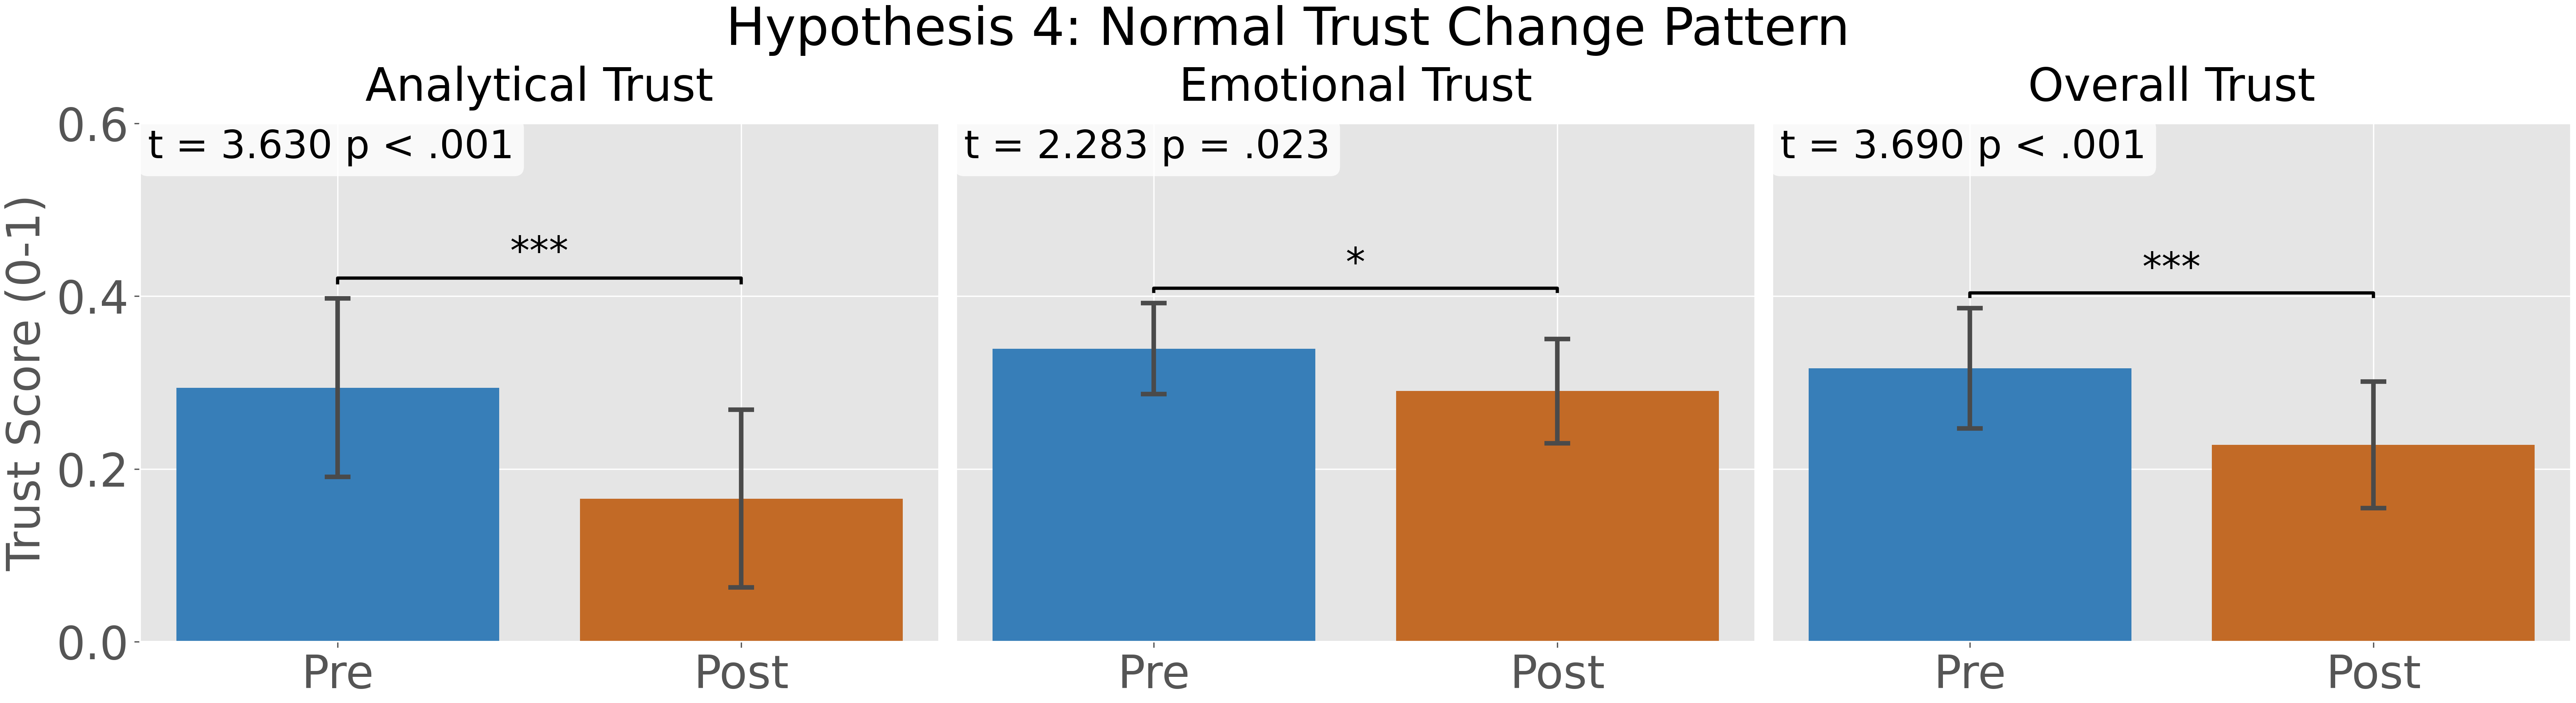
\includegraphics[width=\linewidth]{Figures/hypothesis4.png}

\captionof{figure}{Visualization for Hypothesis 4.}
\label{fig:hypothesis4}
\end{center}

Hypothesis 4 tested whether Normal participants showed a distinct trust-change pattern across analytical, emotional, and overall trust. Figure \ref{fig:hypothesis4} summarizes these three pre-post tests. Across $304$ Normal participants, analytical trust decreased from $M_{pre}=0.294$ (95\% CI [0.191, 0.397]) to $M_{post}=0.166$ (95\% CI [0.063, 0.269]), $t(303)=3.630$, $p < .001$, $W=13264.500$, $p_{W} = .004$, $d=-0.208$, and $\Delta=-0.128$. Emotional trust changed from $M_{pre}=0.339$ (95\% CI [0.286, 0.392]) to $M_{post}=0.290$ (95\% CI [0.230, 0.351]), $t(303)=2.283$, $p = .023$, $W=6912.000$, $p_{W} = .057$, $d=-0.131$, and $\Delta=-0.049$. Overall trust decreased from $M_{pre}=0.317$ (95\% CI [0.247, 0.386]) to $M_{post}=0.228$ (95\% CI [0.155, 0.301]), $t(303)=3.690$, $p < .001$, $W=16044.000$, $p_{W} = .016$, $d=-0.212$, and $\Delta=-0.089$. After Benjamini-Hochberg correction, sub-hypotheses 4.1, 4.2, and 4.3 were significant.

\subsection{Hypothesis 5}
\begin{center}
\centering
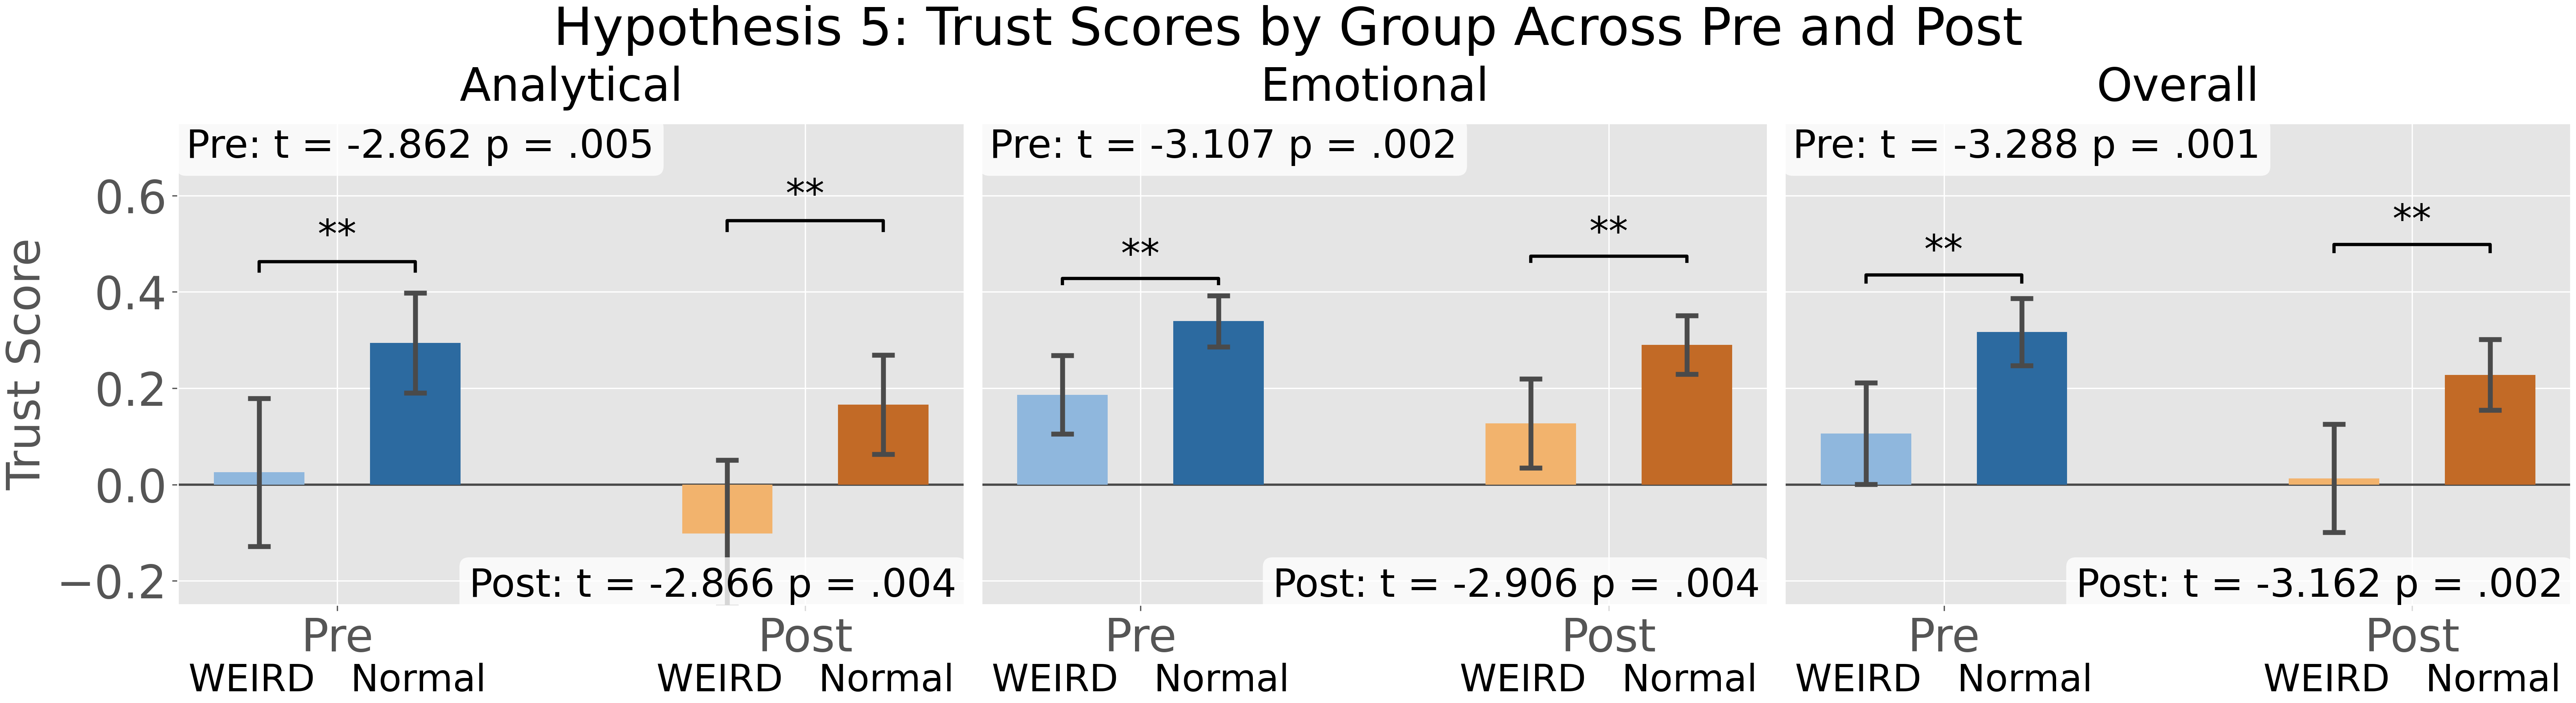
\includegraphics[width=\linewidth]{Figures/hypothesis5.png}

\captionof{figure}{Visualization for Hypothesis 5.}
\label{fig:hypothesis5}
\end{center}

Hypothesis 5 tested whether WEIRD and Normal participants differed in analytical, emotional, and overall trust at the pre- and post-experiment timepoints. Figure \ref{fig:hypothesis5} shows the normalized trust scores for each group, with separate WEIRD-versus-Normal tests at pre and post within each trust domain.

Across WEIRD $ n=150$ and Normal $ n=304$ participants, Analytical pre trust was $M_W=0.025$ (95\% CI [-0.128, 0.179]) for WEIRD participants and $M_N=0.294$ (95\% CI [0.190, 0.398]) for Normal participants, Welch's $t(287.54)=-2.862$, $p = .005$, and $\Delta(M_W-M_N)=-0.269$. Analytical post trust was $M_W=-0.101$ (95\% CI [-0.254, 0.051]) for WEIRD participants and $M_N=0.166$ (95\% CI [0.063, 0.269]) for Normal participants, Welch's $t(288.30)=-2.866$, $p = .004$, and $\Delta(M_W-M_N)=-0.267$.

Emotional pre trust was $M_W=0.187$ (95\% CI [0.105, 0.268]) for WEIRD participants and $M_N=0.339$ (95\% CI [0.286, 0.392]) for Normal participants, Welch's $t(278.80)=-3.107$, $p = .002$, and $\Delta(M_W-M_N)=-0.153$. Emotional post trust was $M_W=0.127$ (95\% CI [0.035, 0.220]) for WEIRD participants and $M_N=0.290$ (95\% CI [0.230, 0.351]) for Normal participants, Welch's $t(280.59)=-2.906$, $p = .004$, and $\Delta(M_W-M_N)=-0.163$.

Overall pre trust was $M_W=0.106$ (95\% CI [0.001, 0.211]) for WEIRD participants and $M_N=0.317$ (95\% CI [0.247, 0.386]) for Normal participants, Welch's $t(282.69)=-3.288$, $p = .001$, and $\Delta(M_W-M_N)=-0.211$. Overall post trust was $M_W=0.013$ (95\% CI [-0.099, 0.125]) for WEIRD participants and $M_N=0.228$ (95\% CI [0.155, 0.301]) for Normal participants, Welch's $t(279.76)=-3.162$, $p = .002$, and $\Delta(M_W-M_N)=-0.215$. After Benjamini-Hochberg correction, sub-hypotheses 5.1, 5.2, 5.3, 5.4, 5.5, and 5.6 were significant.


\subsection{Hypothesis 6}
\begin{center}
\centering
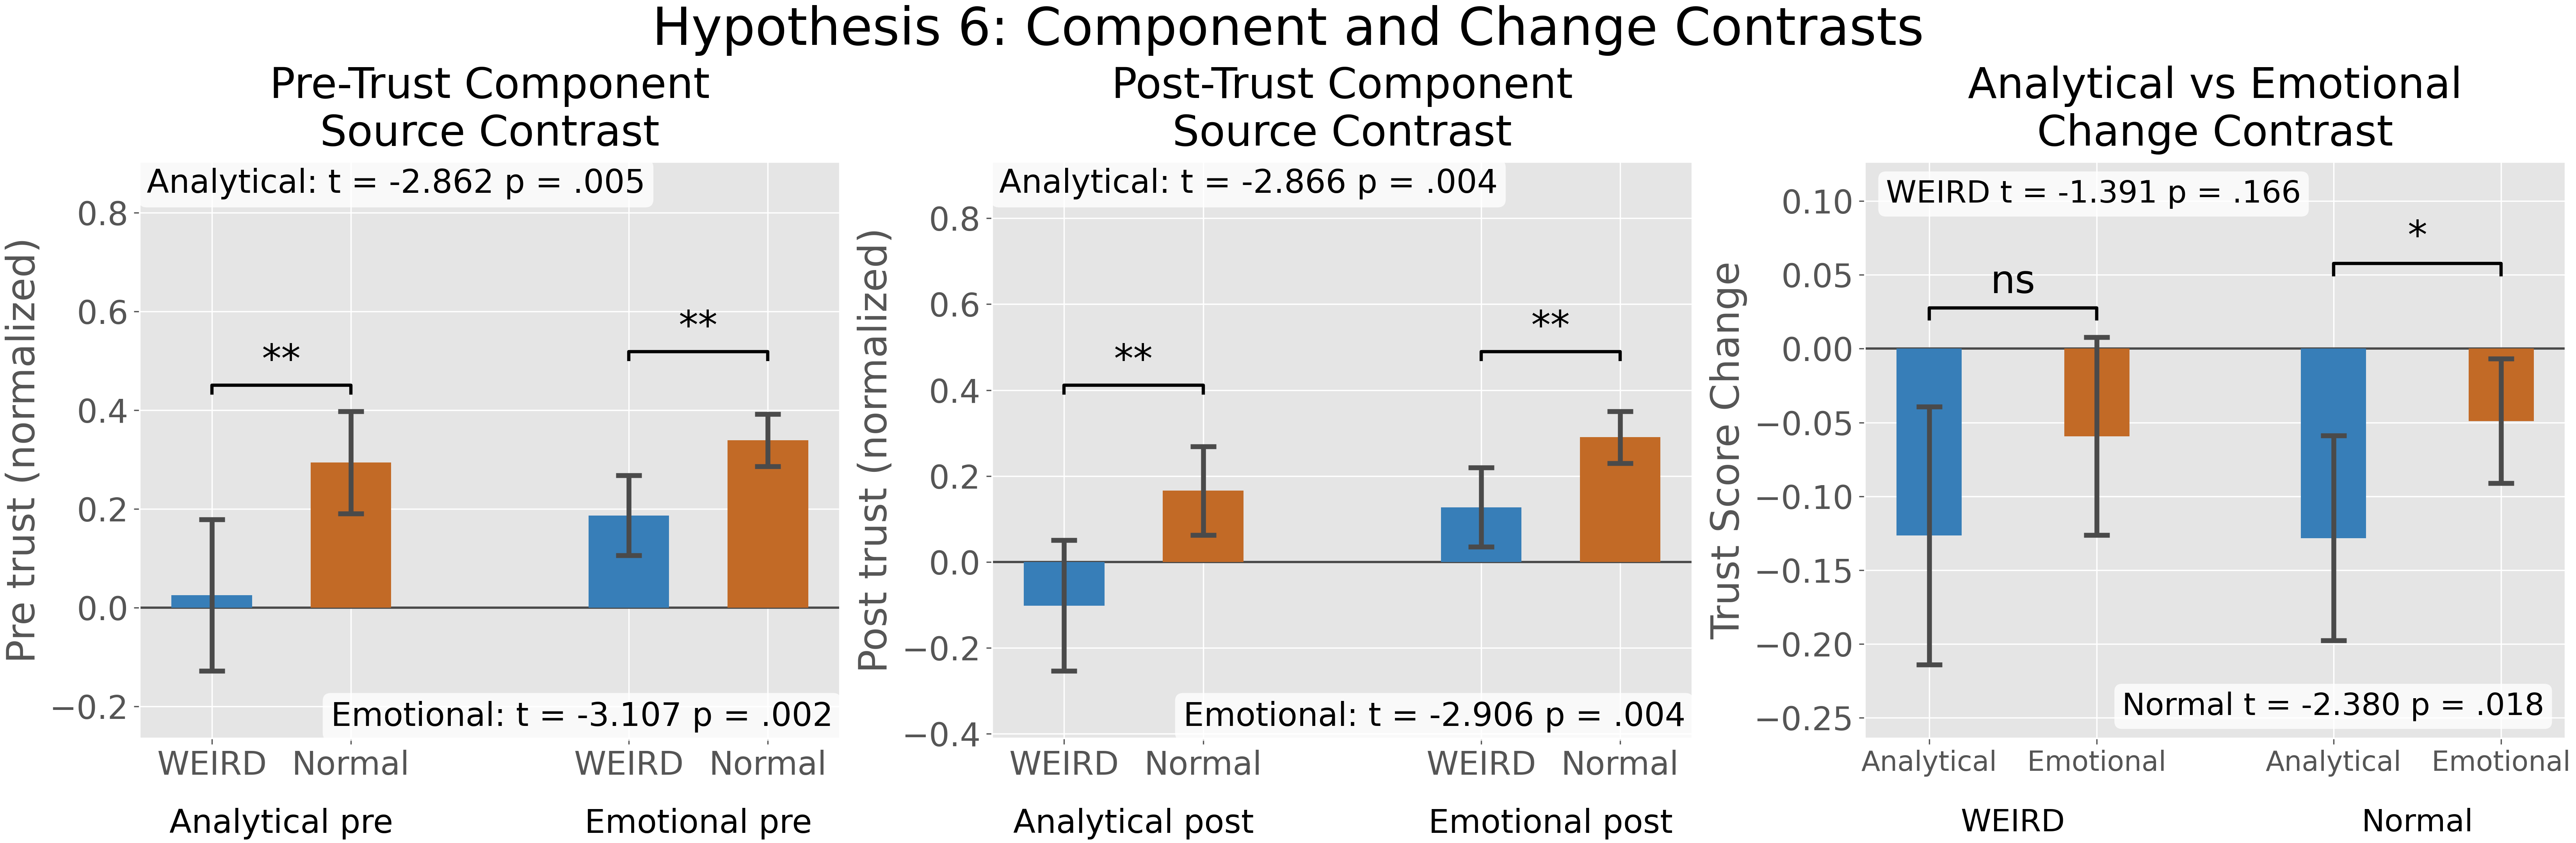
\includegraphics[width=\linewidth]{Figures/hypothesis6.png}

\captionof{figure}{Visualization for Hypothesis 6.}
\label{fig:hypothesis6}
\end{center}
Hypothesis 6 tested whether pre-trust and post-trust component contrasts differed by cultural group, and whether analytical and emotional trust changed by different amounts within each cultural group. The figure includes three analyses in this order: pre-trust component source contrast, post-trust component source contrast, and a single within-group analytical-versus-emotional change contrast. Figure \ref{fig:hypothesis6} summarizes the pre-trust, post-trust, and within-group change contrasts.

Across WEIRD $ n=150$ and Normal $ n=304$ participants, Analytical pre-trust was $M_W=0.025$ (95\% CI [-0.128, 0.179]) for WEIRD participants and $M_N=0.294$ (95\% CI [0.190, 0.398]) for Normal participants, Welch's $t(287.54)=-2.862$, $p = .005$, and $\Delta(M_W-M_N)=-0.269$. Sub-hypothesis 6.1 was statistically significant. Emotional pre-trust was $M_W=0.187$ (95\% CI [0.105, 0.268]) for WEIRD participants and $M_N=0.339$ (95\% CI [0.286, 0.392]) for Normal participants, Welch's $t(278.80)=-3.107$, $p = .002$, and $\Delta(M_W-M_N)=-0.153$. Sub-hypothesis 6.2 was statistically significant. Analytical post-trust was $M_W=-0.101$ (95\% CI [-0.254, 0.051]) for WEIRD participants and $M_N=0.166$ (95\% CI [0.063, 0.269]) for Normal participants, Welch's $t(288.30)=-2.866$, $p = .004$, and $\Delta(M_W-M_N)=-0.267$. Sub-hypothesis 6.3 was statistically significant. Emotional post-trust was $M_W=0.127$ (95\% CI [0.035, 0.220]) for WEIRD participants and $M_N=0.290$ (95\% CI [0.230, 0.351]) for Normal participants, Welch's $t(280.59)=-2.906$, $p = .004$, and $\Delta(M_W-M_N)=-0.163$. Sub-hypothesis 6.4 was statistically significant.

For WEIRD participants ($n=150$), analytical trust change was $M_{A}=-0.127$ (95\% CI [-0.214, -0.039]) and emotional trust change was $M_{E}=-0.059$ (95\% CI [-0.126, 0.008]); the paired comparison yielded $t(149.00)=-1.391$, $p = .166$, and $\Delta(M_A-M_E)=-0.067$. For Normal participants ($n=304$), analytical trust change was $M_{A}=-0.128$ (95\% CI [-0.198, -0.059]) and emotional trust change was $M_{E}=-0.049$ (95\% CI [-0.091, -0.007]); the paired comparison yielded $t(303.00)=-2.380$, $p = .018$, and $\Delta(M_A-M_E)=-0.079$. After Benjamini-Hochberg correction, sub-hypotheses 6.1, 6.2, 6.3, 6.4, and 6.6 were significant, whereas 6.5 was not.

\subsection{Hypotheses Results Summary}
\begin{table}[H]
  \centering
  \caption{Summary of the primary hypothesis tests. Bold values indicate results that remained significant under the Benjamini-Hochberg procedure and conformed to our hypotheses.}
  \label{tab:hypotheses-summary}
\begin{tabular}{||c c c c||} 
     \hline
     Hypothesis  & Test 1 & Test 2 & Test 3 \\ [0.5ex] 
     \hline\hline
     1 & \textbf{Analytical $p<.001$} & \textbf{Emotional $p=.004$} & \textbf{Overall $p<.001$}  \\ 
     \hline
     2 & Analytical $p=.334$ & Emotional $p=.438$ & Overall $p=.283$  \\
     \hline
     2a & \makecell{Overall WEIRD $p=.051$ \\ Overall Normal $p=.985$} & \makecell{Emotional WEIRD $p=.057$ \\ Emotional Normal $p=.630$} & \makecell{Analytical WEIRD $p=.198$ \\ Analytical Normal $p=.751$}  \\
     \hline
     3 & \textbf{Analytical $p=.005$} & Emotional $p=.082$ & \textbf{Overall $p=.003$}  \\
     \hline
    4 & \textbf{Analytical $p<.001$} & \textbf{Emotional $p=.023$} & \textbf{Overall $p<.001$}  \\
     \hline
     5 & \makecell{\textbf{Analytical pre $p=.005$} \\ \textbf{Analytical post $p=.004$}} & \makecell{\textbf{Emotional pre $p=.002$} \\ \textbf{Emotional post $p=.004$}} & \makecell{\textbf{Overall pre $p=.001$} \\ \textbf{Overall post $p=.002$}}  \\ 
     \hline
    6 & \makecell{\textbf{Analytical pre $p=.005$} \\ \textbf{Emotional pre $p=.002$}} & \makecell{\textbf{Analytical post $p=.004$} \\ \textbf{Emotional post $p=.004$}} & \makecell{WEIRD change $p=.166$ \\ \textbf{Normal change $p=.018$}}  \\ [1ex] 
     \hline
\end{tabular}
\end{table}
